\begin{block}{Atomic energy levels}
  \begin{itemize}
  \item A mode-locked laser excites the cesium atoms:
    \begin{itemize}
    \item Spectrum is a series of lines separated by the repetition rate
    \item Wide bandwith, can cover a large number of energy levels
    \end{itemize}
  \end{itemize}
  \begin{columns}
    \begin{column}{0.49\textwidth}
      \begin{figure}
        \begin{center}
          \includegraphics[width=.85\textwidth]{figures/energylevels}
        \end{center}
      \end{figure}
      \begin{itemize}
      \item Coherent population trapping in the hyperfine ground states
      \item Excited state is on the D2 transition
      \item Input light is band-pass filtered to reduce scattered background
      \end{itemize}
    \end{column}
    \begin{column}{0.49\textwidth}
      \begin{figure}
        \begin{center}
          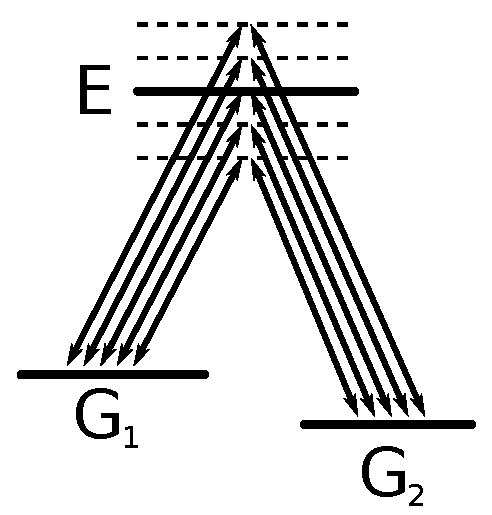
\includegraphics[width=.6\textwidth]{figures/modelockresonance}
        \end{center}
      \end{figure}
      \begin{itemize}
      \item The mode-locked laser have multiple resonance conditions between the excited state ($E$) and the two ground states ($G_1$ and $G_2$)
      \item Interaction is tuned by the repetition rate 
      \end{itemize}
    \end{column}
  \end{columns}
\end{block}
